% =====================================================================
%  Fundamentals of Deep Learning — Class 2 (28 July)
%  Topic (course plan): Introduction to Neural Network
%  Subtopics: Biology NN and Brain; McCulloch-Pitts Neuron,
%             Thresholding and Linear Separability
%
%  Main source: R. Rojas, Neural Networks (Springer, 1996), Ch. 1-2.
%  Supporting: NPTEL Computational Neuroscience notes (ch5, ch6).
%  Figures used with attribution; teaching sequence follows Rojas Ch 1-2.
%
%  Compile:  xelatex main.tex   (run twice)
% =====================================================================
\documentclass[aspectratio=169, 11pt]{beamer}

\usetheme{metropoliscustom}

\usepackage{graphicx}
\DeclareGraphicsExtensions{.pdf,.png,.jpg}
\graphicspath{{figs_official/}{Class02_Intro_Neural_Networks/A_Textbook_Figures/figs_official/}}
\usepackage{amsmath, amssymb}
\usepackage{bm}
\usepackage{tikz}
\usetikzlibrary{arrows.meta, positioning, calc, shapes.misc}
\tcbuselibrary{skins}

\definecolor{bioc}{HTML}{341651}    % biology side (indigo)
\definecolor{modc}{HTML}{800000}    % model side (maroon)

% ---- parallel-teaching strip: Biology (left) vs Model (right)
\newcommand{\biomodel}[2]{%
  \vfill
  {\footnotesize
  \begin{tcolorbox}[enhanced, sidebyside, sidebyside align=top,
                    lefthand ratio=0.485,
                    segmentation style={bioc!35, line width=0.6pt},
                    colback=bioc!5, colframe=bioc!35, boxrule=0.5pt,
                    arc=1.5mm, left=2mm, right=2mm, top=0.8mm, bottom=0.8mm]
    {\color{bioc}\textbf{BIO}}\;\; #1
  \tcblower
    {\color{modc}\textbf{MODEL}}\;\; #2
  \end{tcolorbox}}%
  \vspace{0.6em}%
}

\newcommand{\figsource}[1]{{\scriptsize\color{mcMuted} #1}}

% =====================================================================
\title{Introduction to Neural Networks}
\subtitle{Biology, the McCulloch--Pitts Neuron, and Linear Separability}
\author{Fundamentals of Deep Learning \ \textperiodcentered\ }
\institute{}
\date{}

\footleft{Fundamentals of Deep Learning}
\footright{Introduction to Neural Networks}
\titlelogos{}

\begin{document}

\maketitle

\begin{frame}{Outline}
  \tableofcontents
\end{frame}

% =====================================================================
\section{The Biological Neuron}
% =====================================================================

\begin{frame}{The brain as an inspiration}
  \begin{itemize}
    \item The brain: roughly $10^{11}$ neurons, each connected
          to up to $10^{4}$ others --- massively
          \alert{parallel}, not sequential
    \item Slow components ($\sim$ms switching) yet faster than
          any computer at perception and motor control
    \item Rojas: artificial neural networks are best understood
          as \alert{networks of primitive functions} ---
          simple units, wired together
          \hfill{\scriptsize Rojas (1996), \S1.3}
  \end{itemize}
  \vspace{0.4em}
  \begin{redhighlight}
    The plan: abstract the essential behaviour of a neuron
    into a simple computing unit, then study what networks of
    such units can do.
  \end{redhighlight}
\end{frame}

\begin{frame}{Anatomy of a neuron}
  \centering
  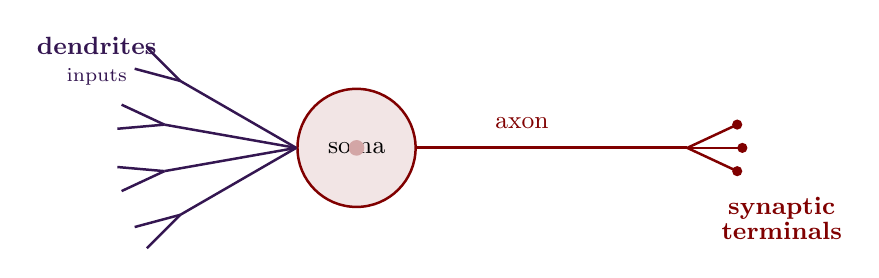
\begin{tikzpicture}[>=Stealth, line width=0.9pt, scale=1.0]
    % soma
    \node[circle, draw=modc, fill=modc!10, minimum size=1.5cm]
      (soma) at (0,0) {\small soma};
    % dendrites (left)
    \foreach \a in {150,170,190,210}{
      \draw[bioc] (soma.west) -- ++(\a:1.7);
      \draw[bioc] ($(soma.west)+(\a:1.7)$) -- ++(\a+15:0.6);
      \draw[bioc] ($(soma.west)+(\a:1.7)$) -- ++(\a-15:0.6);
    }
    \node[bioc, align=center] at (-3.3,1.1)
      {\small\textbf{dendrites}\\[-2pt]{\scriptsize inputs}};
    % axon (right)
    \draw[modc, line width=1.1pt] (soma.east) -- (4.2,0);
    \node[modc] at (2.1,0.32) {\small axon};
    % terminals
    \foreach \a in {25,0,-25}{
      \draw[modc] (4.2,0) -- ++(\a:0.7);
      \node[circle, fill=modc, minimum size=2pt, inner sep=1.3pt]
        at ($(4.2,0)+(\a:0.7)$) {};
    }
    \node[modc, align=center] at (5.4,-0.9)
      {\small\textbf{synaptic}\\[-3pt]\small\textbf{terminals}};
    % nucleus
    \node[circle, fill=modc!35, minimum size=4pt, inner sep=2pt]
      at (0,0) {};
  \end{tikzpicture}
  \vspace{0.5em}
  \begin{itemize}\setlength{\itemsep}{1pt}
    \item \alert{Dendrites} collect incoming signals;
          the \alert{soma} integrates them
    \item If the integrated signal crosses a threshold, the
          neuron \alert{fires} an impulse down the \alert{axon}
    \item \alert{Synapses} pass the signal on --- some
          excitatory, some inhibitory
          \hfill{\scriptsize Rojas (1996), \S1.2}
  \end{itemize}
\end{frame}

\begin{frame}{Firing: an all-or-nothing threshold}
  \begin{itemize}
    \item A neuron integrates its inputs; when the membrane
          potential exceeds a \alert{threshold}, it emits an
          \alert{action potential} --- otherwise it stays
          silent
    \item The spike is \alert{all-or-nothing}: its shape does
          not encode magnitude --- only \emph{whether} and
          \emph{how often} the neuron fires
    \item This thresholding behaviour is the single feature we
          will keep in our first model
          \hfill{\scriptsize cf.\ NPTEL Comp.\ Neuroscience,
          simple neuron models}
  \end{itemize}
  \biomodel{membrane potential crosses a threshold $\to$
            spike}
           {weighted sum crosses a threshold $\to$ output
            $1$}
\end{frame}

\begin{frame}{How the signal travels: the action potential}
  \centering
  \begin{tikzpicture}[line width=1.0pt, xscale=0.78, yscale=0.62]
    \draw[->] (-0.3,0) -- (7.6,0) node[right, font=\scriptsize] {time};
    \draw[->] (0,-1.1) -- (0,2.1)
      node[above, font=\scriptsize, align=center]
      {membrane\\potential};
    \draw[bioc] (0,-0.4) -- (2,-0.4);
    \draw[mcMuted, dashed] (0,0.4) -- (7.4,0.4)
      node[right, font=\scriptsize, mcMuted] {threshold};
    \draw[modc, line width=1.2pt]
      (2,-0.4) -- (2.6,0.4) -- (3.0,1.8) -- (3.4,-0.9)
      -- (3.9,-0.4) -- (7.2,-0.4);
    \node[modc, font=\scriptsize] at (3.2,1.75) {spike};
    \node[bioc, font=\scriptsize] at (1.0,-0.72) {resting};
  \end{tikzpicture}
  \vspace{0.1em}
  \begin{itemize}\setlength{\itemsep}{0pt}
    \item Below threshold, nothing happens; \alert{cross it}
          and the neuron fires a sharp, stereotyped pulse
    \item The pulse travels down the axon \alert{without
          losing strength} --- a digital signal on a noisy wire
    \item After firing, a brief \alert{refractory} dip: the
          neuron resets before it can fire again
          \hfill{\scriptsize Rojas (1996), \S1.2.2}
  \end{itemize}
\end{frame}

\begin{frame}{At the synapse: adding and subtracting}
  \begin{itemize}
    \item Neurons meet at \alert{synapses}; a spike releases
          chemical messengers that nudge the next neuron
    \item \alert{Excitatory} synapses push the membrane
          \emph{toward} threshold; \alert{inhibitory} synapses
          push it \emph{away}
    \item The soma continuously \alert{sums} these pushes ---
          thousands of them --- and fires only if the net
          effect clears the threshold
    \item A single strong inhibitory input can \alert{veto}
          many excitatory ones
          \hfill{\scriptsize Rojas (1996), \S1.2.3}
  \end{itemize}
  \biomodel{excitatory $+$, inhibitory $-$, integrated at the
            soma}
           {positive and negative \alert{weights}, summed in
            the unit}
\end{frame}

% =====================================================================
\section{From Neuron to Computing Unit}
% =====================================================================

\begin{frame}{The abstract neuron}
  \begin{columns}[T, onlytextwidth]
    \begin{column}{0.52\textwidth}
      \centering
      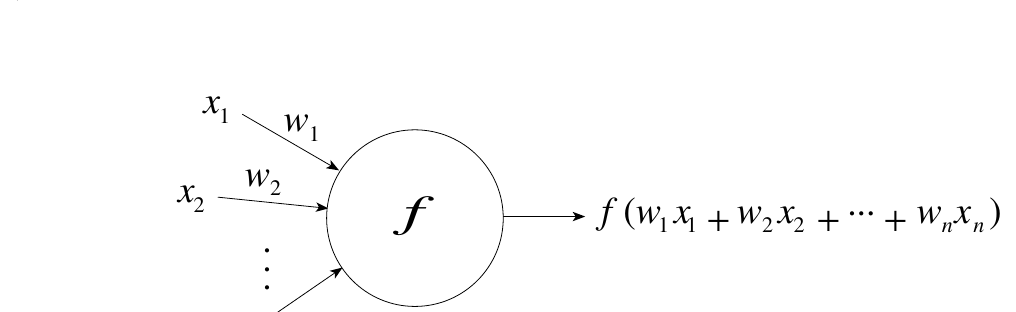
\includegraphics[width=\linewidth]{abstract_neuron}
      \\[0.2em]
      \figsource{Rojas (1996), Fig.~1.14.}
    \end{column}
    \hfill
    \begin{column}{0.44\textwidth}
      \vspace{0.3em}
      \begin{itemize}\setlength{\itemsep}{2pt}
        \item Each input channel $i$ carries a value $x_i$,
              scaled by a \alert{weight} $w_i$
        \item The body integrates the inputs (usually a sum)
              and applies a \alert{primitive function} $f$
        \item Output:
              $f\!\big(w_1x_1+\cdots+w_nx_n\big)$
      \end{itemize}
    \end{column}
  \end{columns}
  \biomodel{dendrites $\times$ synaptic strengths, summed at
            the soma}
           {inputs $x_i$ $\times$ weights $w_i$, summed in the
            unit}
\end{frame}

\begin{frame}{Networks of primitive functions}
  \begin{itemize}
    \item An artificial neural network is nothing but a
          \alert{network of primitive functions}
          \hfill{\scriptsize Rojas (1996), \S1.3.1}
    \item Models differ only in three choices:
  \end{itemize}
  \vspace{0.3em}
  \centering
  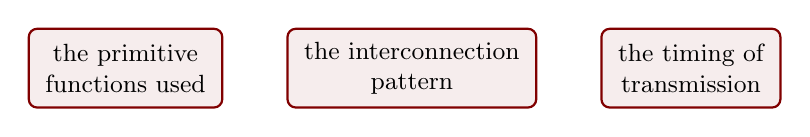
\begin{tikzpicture}[>=Stealth, line width=0.8pt, node distance=4mm,
      b/.style={rounded corners=3pt, draw=modc, fill=modc!7,
                align=center, minimum height=1.0cm,
                inner xsep=6pt, font=\small}]
    \node[b] (a) {the \alert{primitive}\\functions used};
    \node[b, right=8mm of a] (b) {the \alert{interconnection}\\pattern};
    \node[b, right=8mm of b] (c) {the \alert{timing} of\\transmission};
  \end{tikzpicture}
  \vspace{0.4em}
  \begin{itemize}
    \item Today's primitive function: the simplest possible ---
          a \alert{threshold}
  \end{itemize}
\end{frame}

\begin{frame}{Networks can approximate functions}
  \begin{columns}[T, onlytextwidth]
    \begin{column}{0.46\textwidth}
      \centering
      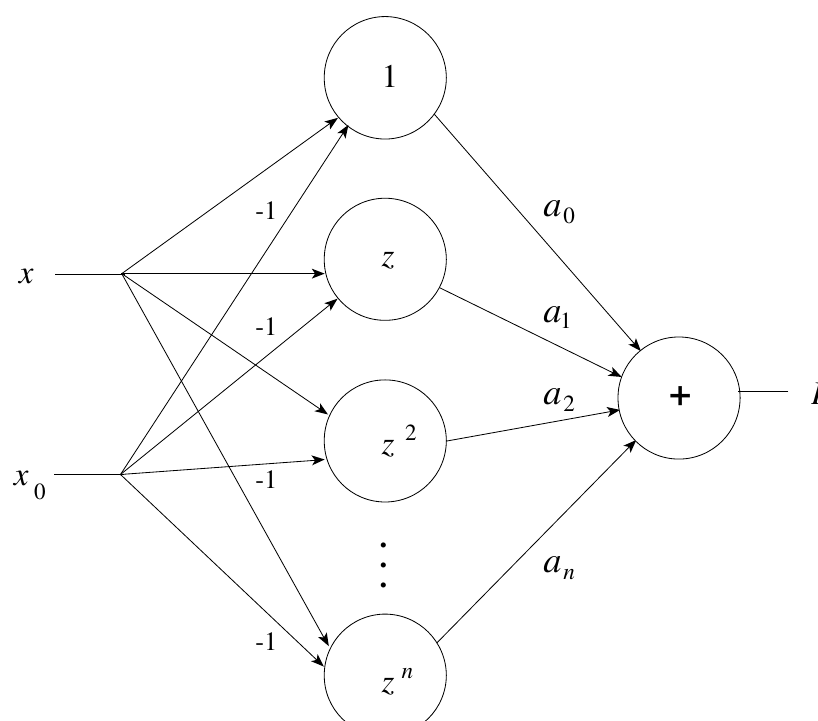
\includegraphics[height=0.5\textheight]{taylor_net}
      \\[0.1em]
      \figsource{Rojas (1996), Fig.~1.16: a Taylor network.}
    \end{column}
    \hfill
    \begin{column}{0.5\textwidth}
      \vspace{0.3em}
      \begin{itemize}\setlength{\itemsep}{2pt}
        \item Choose the primitive functions as powers
              $z,z^2,\dots,z^n$ and the network computes a
              \alert{Taylor series}
        \item Choose sines and it computes a \alert{Fourier
              series} instead
        \item The lesson: a network is a \alert{function
              approximator} --- its power comes from
              \emph{which} primitives you compose and how
        \item The weights $a_0,\dots,a_n$ can even be
              \alert{learned} from data
              \hfill{\scriptsize Rojas (1996), \S1.3.2}
      \end{itemize}
    \end{column}
  \end{columns}
\end{frame}

% =====================================================================
\section{The McCulloch--Pitts Unit}
% =====================================================================

\begin{frame}{Feed-forward vs.\ recurrent}
  \centering
  \begin{tikzpicture}[>=Stealth, line width=0.9pt,
      u/.style={circle, draw, minimum size=6mm, inner sep=0pt,
                font=\scriptsize}]
    % feed-forward
    \begin{scope}
      \node[u, draw=modc, fill=modc!8] (a1) at (0,0.6) {};
      \node[u, draw=modc, fill=modc!8] (a2) at (0,-0.6) {};
      \node[u, draw=modc, fill=modc!8] (b1) at (1.5,0) {};
      \node[u, draw=modc, fill=modc!8] (c1) at (3.0,0) {};
      \draw[->] (a1)--(b1); \draw[->] (a2)--(b1); \draw[->] (b1)--(c1);
      \node[font=\small\bfseries, modc] at (1.5,-1.5) {feed-forward};
      \node[font=\scriptsize, mcMuted] at (1.5,-2.0)
        {flows one way, no cycles};
    \end{scope}
    % recurrent
    \begin{scope}[xshift=6.2cm]
      \node[u, draw=bioc, fill=bioc!8] (r1) at (0,0.5) {};
      \node[u, draw=bioc, fill=bioc!8] (r2) at (1.6,0.5) {};
      \node[u, draw=bioc, fill=bioc!8] (r3) at (0.8,-0.7) {};
      \draw[->] (r1)--(r2); \draw[->] (r2)--(r3);
      \draw[->] (r3)--(r1);
      \node[font=\small\bfseries, bioc] at (0.8,-1.5) {recurrent};
      \node[font=\scriptsize, mcMuted] at (0.8,-2.0)
        {has cycles: memory};
    \end{scope}
  \end{tikzpicture}
  \vspace{0.5em}
  \begin{itemize}\setlength{\itemsep}{1pt}
    \item \alert{Feed-forward}: a directed acyclic graph ---
          output is a fixed function of the input
    \item \alert{Recurrent}: cycles let signals loop back,
          giving the network \alert{state} and memory
    \item Chapters 2--7 (and this course) focus on
          feed-forward networks
          \hfill{\scriptsize Rojas (1996), \S2.1.1}
  \end{itemize}
\end{frame}

\begin{frame}{The McCulloch--Pitts unit (1943)}
  \begin{columns}[T, onlytextwidth]
    \begin{column}{0.46\textwidth}
      \centering
      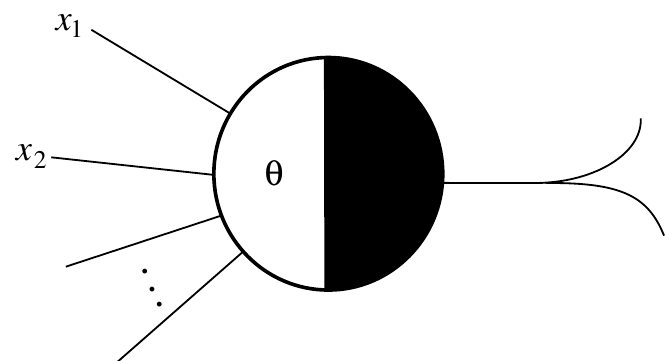
\includegraphics[width=0.92\linewidth]{mp_unit}
      \\[0.2em]
      \figsource{Rojas (1996), Fig.~2.6.}
    \end{column}
    \hfill
    \begin{column}{0.5\textwidth}
      \vspace{0.3em}
      \begin{itemize}\setlength{\itemsep}{2pt}
        \item Inputs and output are \alert{binary}
              ($0$ or $1$); edges are unweighted
        \item Edges are \alert{excitatory} or
              \alert{inhibitory} (small circle)
        \item Each unit has a threshold $\theta$; drawn as a
              circle with a black half
              \hfill{\scriptsize Minsky's convention}
      \end{itemize}
    \end{column}
  \end{columns}
  \biomodel{excitatory / inhibitory synapses}
           {excitatory / inhibitory edges into a threshold
            unit}
\end{frame}

\begin{frame}{The firing rule}
  A unit receives $x_1,\dots,x_n$ on $n$ excitatory edges and
  $y_1,\dots,y_m$ on $m$ inhibitory edges
  (Rojas, 1996, \S2.1):
  \vspace{0.1em}
  \begin{itemize}\setlength{\itemsep}{1pt}
    \item If $m\ge 1$ and \alert{any} inhibitory signal
          $y_j = 1$: the unit is \alert{inhibited},
          output $=0$
    \item Otherwise compute $x = x_1+\cdots+x_n$ and compare
          with $\theta$:
          $\quad\text{output}=1$ if $x\ge\theta$, else $0$
    \item With no inhibition, the unit acts as a
          \alert{threshold gate}
  \end{itemize}
  \biomodel{fire iff input exceeds threshold; inhibition can
            veto}
           {output $1$ iff $x\ge\theta$; any active inhibitor
            forces $0$}
\end{frame}

\begin{frame}{The activation is a step function}
  \begin{columns}[T, onlytextwidth]
    \begin{column}{0.5\textwidth}
      \centering
      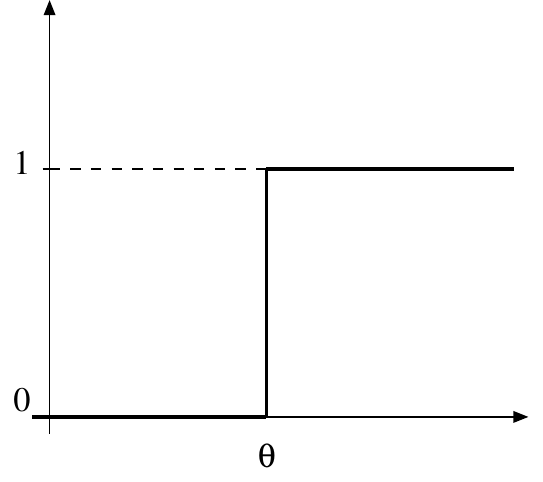
\includegraphics[height=0.46\textheight]{step_fn}
      \\[0.15em]
      \figsource{Rojas (1996), Fig.~2.7.}
    \end{column}
    \hfill
    \begin{column}{0.46\textwidth}
      \vspace{0.4em}
      \begin{itemize}\setlength{\itemsep}{2pt}
        \item The output jumps \alert{discontinuously} from
              $0$ to $1$ at $x=\theta$
        \item This is the \alert{step} (Heaviside)
              activation function
        \item Its hard threshold mirrors the neuron's
              all-or-nothing spike
      \end{itemize}
    \end{column}
  \end{columns}
  \biomodel{action potential: all-or-nothing}
           {step function: output flips at $\theta$}
\end{frame}

% =====================================================================
\section{Computing with Threshold Logic}
% =====================================================================

\begin{frame}{Boolean functions from threshold gates}
  \begin{columns}[T, onlytextwidth]
    \begin{column}{0.5\textwidth}
      \centering
      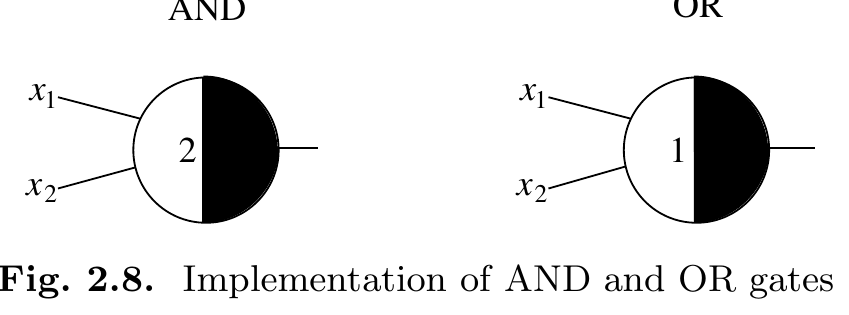
\includegraphics[width=\linewidth]{and_or}
      \\[0.15em]
      \figsource{Rojas (1996), Fig.~2.8.}
    \end{column}
    \hfill
    \begin{column}{0.46\textwidth}
      \vspace{0.3em}
      {\small Two inputs, associate $1=\textit{true}$,
      $0=\textit{false}$:}
      \begin{itemize}\setlength{\itemsep}{2pt}
        \item \alert{AND}: threshold $\theta=2$ --- fires
              only if \emph{both} inputs are $1$
        \item \alert{OR}: threshold $\theta=1$ --- fires if
              \emph{either} input is $1$
      \end{itemize}
      {\small A single unit already computes fundamental
      logic gates.}
    \end{column}
  \end{columns}
  \biomodel{a neuron as a coincidence detector}
           {a threshold gate computing AND / OR}
\end{frame}

\begin{frame}{Threshold logic is expressive}
  \begin{itemize}
    \item A single unit can compute AND or OR of \alert{$n$
          arguments} --- just set $\theta = n$ (AND) or
          $\theta = 1$ (OR)
    \item Negation needs an \alert{inhibitory} edge: a unit
          with $\theta = 0$ and one inhibitory input computes
          NOT
    \item With AND, OR, and NOT available, threshold-logic
          networks can compute \alert{any Boolean function}
          \hfill{\scriptsize Rojas (1996), \S2.2}
  \end{itemize}
  \vspace{0.3em}
  \begin{redhighlight}
    But how expressive is a \emph{single} unit? The answer is
    geometric.
  \end{redhighlight}
\end{frame}

\begin{frame}{Any Boolean function, by construction}
  A logical function is a \alert{table}: for each input
  vector, a $0$ or a $1$. To build a network for it
  (Rojas, 1996, \S2.2.3):
  \vspace{0.2em}
  \begin{enumerate}\setlength{\itemsep}{2pt}
    \item For every input row that should output $1$, use one
          unit as a \alert{decoder} --- it fires \emph{only}
          for that exact vector
    \item A decoder for $(1,0,1)$: excitatory edges from the
          $1$-bits, inhibitory from the $0$-bits, threshold
          $=$ number of $1$-bits
    \item Feed all decoders into a single \alert{OR} unit
  \end{enumerate}
  \vspace{0.3em}
  \begin{redhighlight}
    Two layers of threshold units suffice for \emph{any}
    Boolean function --- expressive power is not the problem.
  \end{redhighlight}
\end{frame}

% =====================================================================
\section{Geometry: Linear Separability}
% =====================================================================

\begin{frame}{A unit splits input space into half-spaces}
  \begin{columns}[T, onlytextwidth]
    \begin{column}{0.46\textwidth}
      \centering
      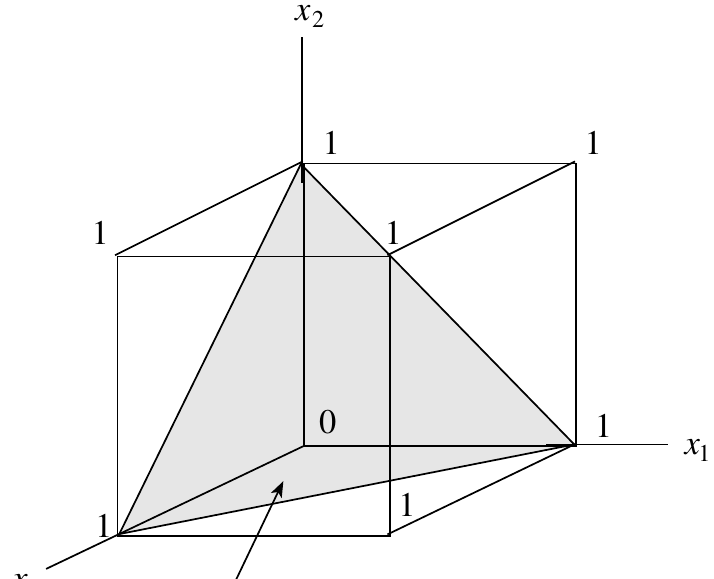
\includegraphics[height=0.46\textheight]{sep_or}
      \\[0.15em]
      \figsource{Rojas (1996), Fig.~2.12: the OR function.}
    \end{column}
    \hfill
    \begin{column}{0.50\textwidth}
      {\small For input $(x_1,x_2,x_3)$ and threshold
      $\theta$, the unit tests $x_1{+}x_2{+}x_3 \ge \theta$:}
      \begin{itemize}\setlength{\itemsep}{1pt}
        \item The equality $x_1{+}x_2{+}x_3=\theta$ is a
              \alert{separating plane}
        \item One side fires ($1$), the other does not ($0$)
        \item OR: $\theta=1$; only the all-zero vertex lies
              below the plane
      \end{itemize}
    \end{column}
  \end{columns}
  \biomodel{a neuron responds to a region of stimulus space}
           {a unit responds to a \emph{half-space} of inputs}
\end{frame}

\begin{frame}{Parallel planes, different thresholds}
  \begin{columns}[T, onlytextwidth]
    \begin{column}{0.48\textwidth}
      \centering
      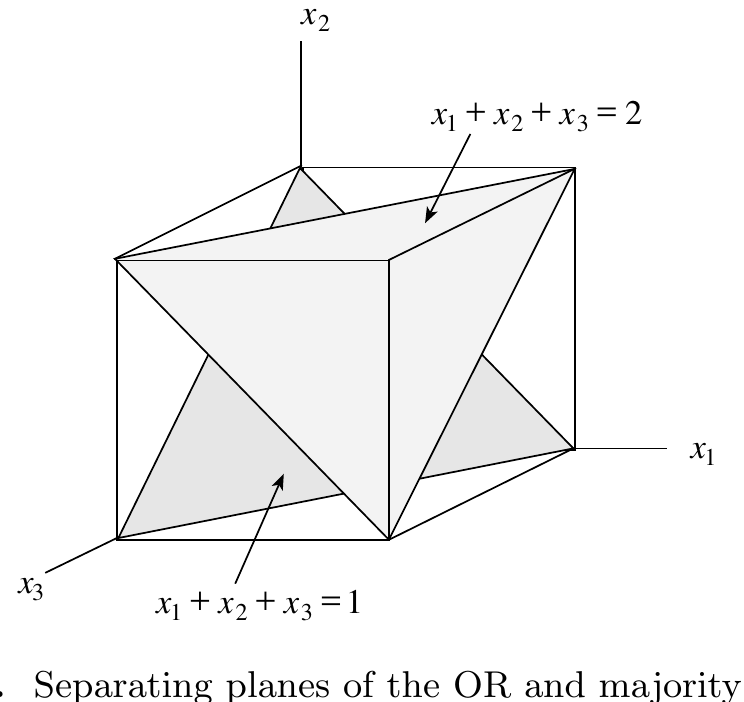
\includegraphics[height=0.52\textheight]{sep_planes}
      \\[0.15em]
      \figsource{Rojas (1996), Fig.~2.13: OR and majority.}
    \end{column}
    \hfill
    \begin{column}{0.48\textwidth}
      \vspace{0.3em}
      \begin{itemize}\setlength{\itemsep}{2pt}
        \item \alert{OR}: plane $x_1{+}x_2{+}x_3=1$
        \item \alert{Majority}: plane $x_1{+}x_2{+}x_3=2$
              --- fires when at least two inputs are $1$
        \item For McCulloch--Pitts units (unit weights) the
              separating planes are always \alert{parallel}
        \item \alert{Non-parallel} planes require
              \alert{weighted} edges --- the perceptron
              (Class 3)
      \end{itemize}
    \end{column}
  \end{columns}
\end{frame}

\begin{frame}{The one it cannot do: XOR}
  \begin{columns}[T, onlytextwidth]
    \begin{column}{0.44\textwidth}
      \centering
      \begin{tikzpicture}[line width=0.9pt, scale=2.1]
        \draw[->] (-0.2,0) -- (1.35,0) node[right,font=\scriptsize]{$x_1$};
        \draw[->] (0,-0.2) -- (0,1.35) node[above,font=\scriptsize]{$x_2$};
        % class 0 (output 0): (0,0) and (1,1) -- blue circles
        \node[circle, draw=bioc, fill=bioc!15, minimum size=5pt,
              inner sep=1.5pt] at (0,0) {};
        \node[circle, draw=bioc, fill=bioc!15, minimum size=5pt,
              inner sep=1.5pt] at (1,1) {};
        % class 1 (output 1): (0,1) and (1,0) -- maroon crosses
        \node[modc, font=\normalsize] at (0,1) {$\bm\times$};
        \node[modc, font=\normalsize] at (1,0) {$\bm\times$};
        \node[font=\scriptsize] at (-0.13,-0.13) {$0$};
        \node[font=\scriptsize] at (1.13,1.13) {$1$};
        % a couple of failed separating lines
        \draw[mcMuted, dashed] (-0.15,0.55) -- (1.2,0.75);
        \draw[mcMuted, dashed] (0.35,-0.15) -- (0.65,1.25);
      \end{tikzpicture}
      \\[0.2em]
      \figsource{$\bm\times$: XOR $=1$;\;
      $\circ$: XOR $=0$.}
    \end{column}
    \hfill
    \begin{column}{0.5\textwidth}
      \vspace{0.4em}
      \begin{itemize}\setlength{\itemsep}{2pt}
        \item XOR outputs $1$ when the inputs \alert{differ},
              $0$ when they agree
        \item The two $\times$ points sit on \alert{opposite
              corners} --- so do the two $\circ$ points
        \item \alert{No single straight line} can put both
              $\times$ on one side and both $\circ$ on the
              other
        \item XOR is \alert{not linearly separable} --- a wall
              a single unit cannot climb
      \end{itemize}
    \end{column}
  \end{columns}
\end{frame}

\begin{frame}{Linear separability --- and its limit}
  \begin{itemize}
    \item A single threshold unit can compute exactly the
          \alert{linearly separable} functions: those whose
          $1$- and $0$-inputs can be split by a hyperplane
    \item AND, OR, majority --- all linearly separable
    \item XOR is not --- and most functions of many variables
          are not, either
  \end{itemize}
  \vspace{0.3em}
  \begin{redhighlight}
    A single unit is a linear classifier. Escaping
    linear separability needs \alert{weights} (Class 3) and,
    ultimately, \alert{layers} (Classes 5--7).
  \end{redhighlight}
\end{frame}

\begin{frame}{Takeaways}
  \begin{enumerate}\setlength{\itemsep}{2pt}
    \item A neuron integrates weighted inputs and fires when a
          \alert{threshold} is crossed --- all-or-nothing
    \item The \alert{McCulloch--Pitts unit} keeps only this:
          binary inputs, a threshold, excitatory/inhibitory
          edges
    \item A single unit computes AND, OR, majority --- but
          only \alert{linearly separable} functions
    \item Geometrically it is a \alert{separating hyperplane};
          XOR already escapes it
  \end{enumerate}
  \vspace{0.3em}
  \begin{redhighlight}
    Class~3: add \alert{weights} and a \alert{learning rule}
    --- the perceptron.
  \end{redhighlight}
\end{frame}

\begin{frame}{References}
  \footnotesize
  \begin{itemize}
    \item R.~Rojas. \textit{Neural Networks: A Systematic
          Introduction.} Springer, 1996. Chapters 1--2.
          Figures 1.14, 2.6, 2.7, 2.8, 2.12, 2.13 reproduced
          with attribution.
    \item W.~S.~McCulloch \& W.~Pitts (1943). ``A logical
          calculus of the ideas immanent in nervous
          activity.'' \textit{Bulletin of Mathematical
          Biophysics}, 5, 115--133.
    \item NPTEL Computational Neuroscience notes (simplified
          neuron models; perceptrons), used for supporting
          intuition.
  \end{itemize}
\end{frame}

\begin{frame}[standout]
  Questions?
\end{frame}

\end{document}
